\documentclass[30pt,twocolumn,letterpaper]{article}
\usepackage{cvpr}
\usepackage{times}
\usepackage{booktabs}
\usepackage{epsfig}
\usepackage{graphicx}
\usepackage{amsmath}
\usepackage{amssymb}
\cvprfinalcopy
\def\cvprPaperID{****}
\def\httilde{\mbox{\tt\raisebox{-.5ex}{\symbol{126}}}}
\usepackage{graphicx}
\usepackage{indentfirst}
\setlength{\parindent}{2em}
\usepackage{cite}
\usepackage[colorlinks,linkcolor=red,anchorcolor=blue,citecolor=green,backref=page]{hyperref}
\author{Qilei Zhang\\\\
Jun 22 2018}
\title{Neural Turing Machines}
\begin{document}
\maketitle
\begin{abstract}
  The ability of neural networks can be extended by coupling them to external memory resources, which can interact through the attention process.
\end{abstract}
\section{Introduction}
Computer programs take advantage of three basic mechanisms: basic operations, logical flow control and external memory, which can be written and read in the process of computing. Despite its success in simulating complex data, modern machine learning largely ignores the use of logical flow control and external memory\cite{Arbib1961Turing}. \\
\begin{figure}[htbp]
\small
\centering
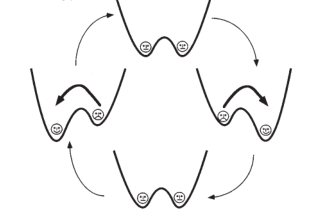
\includegraphics[width=20em]{000.png}
\caption{Neural Turing Machine Architecture.}
\label{fig:lable}
\end{figure}\\
\section{Foundational Research}
The concept of working memory is most developed in psychology, explaining the implementation of tasks involving short-term information manipulation. Psychologists have extensively studied the capacity limitation of working memory\cite{Moore1997Quantum}, which is usually quantified by the number of "blocks" of easily recalled information. These capacity constraints lead to understanding structural constraints in the human working memory system, but we are delighted to exceed them in our own work\cite{Wells1998Turing}.\\
\begin{figure}[htbp]
\small
\centering
\includegraphics[width=20em]{001.png}
\caption{Copy Learning Curves.}
\label{fig:lable}
\end{figure}\\
\section{Experiments}
The initial experimental purpose of copying and sorting data sequences is not only to build NTM to solve problems, but also to do so through learning compact internal procedures. The characteristic of such a solution is that they extend far beyond the scope of training data\cite{Yu2015Empirical}.
{\small
\bibliographystyle{ieee}
\bibliography{1}
}
\end{document}
